\begin{frame}
  \frametitle{3D Point to Pixel: Estimating the Parameters of P}
  \begin{equation*}
    \underset{\substack{\text{pixel}\\ \text{coordinate}}}{\mathbf{x}} \sim \underset{\substack{\text{trans-}\\ \text{formation}}}{\mathbf{P}}
    \underset{\substack{\text{world}\\ \text{coordinate}}}{\mathbf{X}}
  \end{equation*}  
\end{frame}

\begin{frame}
  \frametitle{Estimating Camera Parameters Given the Geometry}
  \begin{itemize}
    \item known control points
  \end{itemize}
  \begin{center}
    \includegraphics[width=0.5\columnwidth]{./images/localization_3d_2d.pdf}
  \end{center}
\end{frame}

\begin{frame}
  \frametitle{Estimate Ex- and Intrinsics}
  \begin{itemize}
    \item \textbf{Wanted}: Extrinsic and intrinsic parameters of a camera
    \item \textbf{Given}: Coordinates of object points (control points)
    \item \textbf{Observed}: Coordinates of those known 3D object points in the image
  \end{itemize}
\end{frame}

\begin{frame}
  \frametitle{Mapping}
  Direct linear transform (DLT) maps any object point $\mathbf{X}$ to the image point $\mathbf{x}$.
  \begin{center}
    
\includegraphics[width=0.5\columnwidth]{./images/dlt_3d_2d.pdf}
  \end{center}
%
  \begin{equation*}
    \vec{x} = \projectionMatrix \vec{X} \quad \text{donde} \quad
    \underset{3 \times 4}{\projectionMatrix}=\underset{3 \times 3}{\intrinsicMatrix}\underset{3 \times 4}{\begin{bmatrix} \underset{3 \times 3}{\rotation} & \underset{3 \times 1}{\translation}\end{bmatrix}}
  \end{equation*}
%
\end{frame}

% \begin{frame}
%   \frametitle{Camera Parameters}
%   \begin{itemize}
%     \item Intrinsics -- Camera-internal parameters. Given through $\intrinsicMatrix$.
%     \item Extrinsics -- Pose parameters of the camera. Given through $\rotation$ and $\vec{X}_{0}$.
%     \item Projection matrix $\projectionMatrix$ contains both, the in- and extrinsics.
%   \end{itemize}

%   \begin{align*}
%     \vec{x} &= \projectionMatrix \vec{X}\\
%     \vec{x} &= \intrinsicMatrix \begin{bmatrix} \rotation & \translation \end{bmatrix} \vec{X}\\
%     \vec{x} &= \intrinsicMatrix \rotation \begin{bmatrix} \vec{I} & -\vec{X}_{0} \end{bmatrix} \vec{X}\\
%   \end{align*}
% \end{frame}

\begin{frame}
  \frametitle{Compute the 11 intrinsic and extrinsic parameters}
  Direct Linear Transform (DLT)
  \begin{itemize}
    \item control point coordinates (given)
    \item observed image point  (given)
    \item 3 rotations, 3 translations
    \item 5 intrinsic parameters $(f_{x}, f_{y}, \principalPoint_{x}, \principalPoint_{y}, s)$
  \end{itemize}

  \begin{center}
    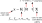
\includegraphics[width=0.5\columnwidth]{./images/projection_matrix_unknowns.pdf}
  \end{center}
\end{frame}

\begin{frame}
  \frametitle{How Many Points Are Needed?}
  Each point gives two observation equations, one for each image coordinate.
  % \includegraphics[width=0.6\textwidth]{placeholder-image.jpg}
\end{frame}

\begin{frame}
  \frametitle{Spatial Resection vs. DLT}
  \begin{itemize}
    \item Calibrated camera: 6 unknowns. Need at least 3 points. Problem solved by spatial resection.
    \item Uncalibrated camera: 11 unknowns. Need at least 6 points (assuming affine camera). Problem solved by DLT.
  \end{itemize}
  % \includegraphics[width=0.6\textwidth]{placeholder-image.jpg}
\end{frame}

\begin{frame}
  \frametitle{DLT: Direct Linear Transform}
  Computing the Orientation of an Uncalibrated Camera using $\ge 6$ known points.
  % \includegraphics[width=0.7\textwidth]{placeholder-image.jpg}
\end{frame}

\begin{frame}
  \frametitle{DLT: Problem Specification}
  \begin{itemize}
    \item Task: Estimate the 11 elements of $P$.
    \item Given: 3D coordinates $\mathbf{X}_i$ of object points.
    \item Observed image coordinates $\mathbf{x}_i$ of an uncalibrated camera.
  \end{itemize}
  % \includegraphics[width=0.7\textwidth]{placeholder-image.jpg}
\end{frame}

\begin{frame}
  \frametitle{Rearrange the DLT Equation}
  Leads to a system of equations, linear in the parameters A, B, C.
  % \includegraphics[width=0.65\textwidth]{placeholder-image.jpg}
\end{frame}

\begin{frame}
  \frametitle{Estimating the Elements of P}
  \begin{itemize}
    \item Collect elements of $P$ into a parameter vector.
    \item Stacking of rows of $P$.
  \end{itemize}
  % \includegraphics[width=0.7\textwidth]{placeholder-image.jpg}
\end{frame}

\begin{frame}
  \frametitle{Solving the Linear System (Homogeneous System => SVD)}
  \begin{itemize}
    \item Solve $A\mathbf{p}=0$ via SVD.
    \item Choose $\mathbf{p}$ as singular vector of smallest singular value.
  \end{itemize}
  % \includegraphics[width=0.6\textwidth]{placeholder-image.jpg}
\end{frame}

\begin{frame}
  \frametitle{Redundant Observations}
  \begin{itemize}
    \item Minimize $\|A\mathbf{p}\|$ with $\|\mathbf{p}\|=1$.
    \item Use SVD to find best solution.
  \end{itemize}
  % \includegraphics[width=0.7\textwidth]{placeholder-image.jpg}
\end{frame}

\begin{frame}
  \frametitle{Critical Surfaces}
  \begin{itemize}
    \item $M$ is of rank 11 if number of points $\ge 6$.
    \item No solution if all points lie on a plane.
  \end{itemize}
  % \includegraphics[width=0.65\textwidth]{placeholder-image.jpg}
\end{frame}

\begin{frame}
  \frametitle{From $P$ to $K,R,t$}
  % \includegraphics[width=0.6\textwidth]{placeholder-image.jpg}
\end{frame}

\begin{frame}
  \frametitle{Decomposition of P}
  \begin{itemize}
    \item Compute $K, R, t$ from $P$.
    \item Use QR decomposition for rotation and calibration matrices.
  \end{itemize}
  % \includegraphics[width=0.7\textwidth]{placeholder-image.jpg}
\end{frame}

\begin{frame}
  \frametitle{DLT in a Nutshell}
  \begin{enumerate}
    \item Build matrix $M$ for linear system $M p = 0$.
    \item Solve by SVD.
    \item Decompose $P$ to obtain $K,R,t$.
  \end{enumerate}
  % \includegraphics[width=0.6\textwidth]{placeholder-image.jpg}
\end{frame}

\begin{frame}
  \frametitle{Discussion DLT}
  \begin{itemize}
    \item Solution unstable if control points nearly planar.
    \item Not statistically optimal.
  \end{itemize}
  % \includegraphics[width=0.7\textwidth]{placeholder-image.jpg}
\end{frame}

\begin{frame}
  \frametitle{Summary}
  \begin{itemize}
    \item Direct linear transform estimates intrinsic and extrinsic camera parameters.
    \item Needs at least 6 control points.
    \item Provides direct solution.
  \end{itemize}
  % \includegraphics[width=0.7\textwidth]{placeholder-image.jpg}
\end{frame}

\begin{frame}
  \frametitle{Literature}
  \begin{itemize}
    \item Förstner \& Wrobel, Photogrammetric Computer Vision, Chapter 11.2
    \item Förstner, Scriptum Photogrammetrie I, Chapter 13.3
  \end{itemize}
  % \includegraphics[width=0.5\textwidth]{placeholder-image.jpg}
\end{frame}

\begin{frame}
  \frametitle{Slide Information}
  \begin{itemize}
    \item Slides created by Cyrill Stachniss for Photogrammetry and Robotics courses.
    \item Acknowledgements and notes in original slides.
  \end{itemize}
  % \includegraphics[width=0.5\textwidth]{placeholder-image.jpg}
\end{frame}

\end{document}



\begin{frame}
  \frametitle{Material: Direct Linear Transform}

  Direct Linear Transform for Camera Calibration and Localization (Cyrill Stachniss)
  \url{https://youtu.be/3NcQbZu6xt8}

  Camera Calibration using Zhang's Method (Cyrill Stachniss)
  \url{https://youtu.be/-9He7Nu3u8s}

  Intrinsic and Extrinsic Matrices | Camera Calibration
  \url{https://youtu.be/2XM2Rb2pfyQ}

\end{frame}
